\documentclass[12pt]{article}
\usepackage[margin=1in]{geometry}
\usepackage[utf8]{inputenc}
\usepackage{setspace}
\onehalfspacing
\usepackage{amsmath, amssymb, amsthm, mathtools}
\usepackage{booktabs}
\usepackage{graphicx}
\usepackage{microtype}
\usepackage[dvipsnames]{xcolor}
\usepackage{siunitx}
\usepackage{enumitem}
\usepackage{titlesec}
\usepackage{natbib}
\usepackage{hyperref}

\titleformat{\section}{\normalfont\Large\bfseries}{\thesection}{0.6em}{}
\titleformat{\subsection}{\normalfont\large\bfseries}{\thesubsection}{0.6em}{}
\setlist{itemsep=2pt, topsep=3pt}

\hypersetup{
  colorlinks=true, linkcolor=blue!50!black,
  urlcolor=blue!50!black, citecolor=blue!50!black,
}

\title{\Large\textbf{Adversarial Nowcasting and Monetary Policy:\\Sign-Flips, Filtering, and the Strategic Attacker}}
\author{John Blakeslee}
\date{April 2026}

\begin{document}
\maketitle

\begin{abstract}
\noindent
Central banks increasingly rely on machine-learning nowcasts of real-time economic activity. These pipelines ingest unvetted internet data and so expose monetary policy to a novel attack surface: deliberate contamination of the signals that shape rate decisions. A 2024--2025 Russian disinformation operation demonstrated industrial-scale data poisoning of large language models; the same techniques can be aimed at Federal Reserve nowcasts. This brief builds a workhorse New Keynesian DSGE with Smets--Wouters frictions and a signal-filtering Fed, then asks two questions. First, how much policy distortion can a persistent attack produce? Second, can filtering defend against it, and under what conditions should the Fed choose to filter? Results: under Smets--Wouters calibration, a sustained attack produces roughly 34 basis points of cumulative policy distortion over eight quarters, several times the distortion implied by a fully forward-looking textbook model. A signal-filtering Fed reduces this damage by 84\% in expected-utility terms but does not deter the attack in the cumulative policy-rate or inflation-variance case; the attacker's optimal strategy is largely invariant to the defense regime. A Fed that believes the probability of an active nowcast attack exceeds roughly 25\% should filter heavily, and this threshold is robust across plausible welfare-weight calibrations at the empirical Phillips slope. The analysis reorders the defense-policy space: detection-latency measures (provenance ledgers, cryptographic signatures at ingestion) are first-order because they target the attacker's most-leveraged variable; filter-based responses are damage mitigation conditional on attack.
\end{abstract}

\section{Introduction}

This brief asks two questions: how much policy distortion can a persistent adversarial attack on central-bank nowcasts produce, and under what conditions should the Fed filter its signals in response? Central banks increasingly use machine-learning nowcasts to bridge the lag between economic reality and official statistics. The Bank for International Settlements' 2024 Annual Report documents the acceleration, and recent BIS and ECB working papers survey how central banks are incorporating generative AI and alternative data into policy-relevant monitoring \citep{bis2024, ecb2024ai, aldasoro2024gen}. The practice trades latency for exposure. Unlike the Bureau of Economic Analysis and the Bureau of Labor Statistics, whose data pipelines are air-gapped and rely on secure reporting channels, the open-web sources that power nowcasts are vulnerable to adversarial tampering.

\paragraph{Threat model.}
The specific attack considered here is data poisoning of a public-data input to the Fed's nowcast stack. The 2024--2025 Russian ``Pravda'' operation demonstrated feasibility in the language-model context: the American Sunlight Project documented 3.6 million auto-generated articles pushed through a content network designed to shift large-language-model outputs, and NewsGuard's 2025 audit found that one-third of the major chatbots tested regurgitated Pravda narratives, citing the network's URLs directly \citep{asp2025, newsguard2025}. Economic nowcasts present a natural next target for a state adversary. The attacker is assumed to be a capable state actor with sustained budget, seeking to push US policy rates in a particular direction. The attack surface is the set of public-web inputs to the Fed's nowcast model: scraped price data, social-media sentiment, card-swipe aggregators, job-posting feeds. The attacker's constraint is detection: sustained, large biases are more likely to be caught by anomaly monitors. The defender's instruments include signal filtering (down-weighting noisy indicators in the policy rule), data-provenance tracking (public logging of ingested inputs, enabling crowd-sourced audit), and cryptographic signing at ingestion (making tampering evident in the audit trail).

\paragraph{Literature.}
The classical literature on monetary policy under noisy information maps directly onto the adversarial case. \citet{orphanides2001} documents that real-time output-gap mismeasurement materially shifts the Taylor rule's prescription, and his sequence of papers establishes that standard deviations of first-revision output gaps can approach 200 basis points \citep{orphanides2001, orphanides2003monetary, orphanides2003historical}. \citet{aoki2003} derives the optimal response to noisy gap and inflation indicators in a forward-looking NK model; the brief's single-gain perception block is a special case of this framework. \citet{svensson2003} formalize the result that optimal policy responsiveness to a noisy indicator decreases as its signal-to-noise ratio deteriorates. \citet{orphanides2007robust} extend this to robust control under imperfect knowledge and adaptive learning. \citet{coibion2012} document information rigidities in inflation expectations, which bear on how forcefully the forward-looking expectations channel in NK models can actually work. \citet{blanchard2013news} develop signal-extraction with noisy news shocks, providing the closest methodological parallel. Work by \citet{nimark2008} and \citet{boivin2006} extends signal-extraction to policy-rule design with real-time data. On the adversarial-ML side, the brief builds on \citet{biggio2018wild} and \citet{steinhardt2017}. The gap this brief fills is the application of signal-extraction monetary economics to a deliberate-adversary setting, with the attacker's persistence and magnitude choices endogenized in a simple game.

\paragraph{Contribution.}
Earlier work (Blakeslee 2025) used a three-equation New Keynesian DSGE to demonstrate a single striking result: a \(+1\) percentage-point attack flipping an expected 50 basis-point hike into a 1--2 basis-point cut. This brief extends that analysis in three directions. First, it rebuilds the model on a workhorse Galí (2008) foundation with Smets--Wouters \citep{smetswouters2007} frictions, validates the Julia port bit-for-bit against the Dynare reference, and shows that the impact sign-flip depends on parameter assumptions that the prior analysis left unexamined. Second, it shows that the underlying attack phenomenon is larger in cumulative terms than the earlier calibration implied, and characterizes the parameter space in which this holds. Third, it endogenizes the attacker's strategy and analyzes the policy-defense tradeoff between naive and filtering Feds, connecting the resulting crossover probability to a concrete decision threshold.

Section~\ref{sec:model} presents the model. Section~\ref{sec:calib} describes the calibration, the Julia port validation, and the MMSE Kalman benchmark for the perception filter. Section~\ref{sec:findings} presents five substantive findings with robustness. Section~\ref{sec:attacker} develops the strategic-attacker game and examines whether the defense results hold across alternative attacker objectives. Section~\ref{sec:policy} draws policy implications and reorders the three defense proposals from earlier analysis. Section~\ref{sec:limits} states limitations.

\section{Model}\label{sec:model}

The structure extends the small-scale forward-looking New Keynesian model of \citet{gali2008} with three Smets--Wouters \citep{smetswouters2007} frictions and a single-gain perception block. All variables are expressed as log-deviations from the zero-inflation steady state. Shocks are indexed by \(t\) and persist through their own AR(1) laws of motion.

\subsection{Hybrid New Keynesian Phillips curve}

With \citet{gali1999} indexation at fraction \(\chi_p\) of firms:
\begin{equation}
\pi_t = \frac{\beta}{1 + \beta \chi_p} \mathbb{E}_t[\pi_{t+1}] + \frac{\chi_p}{1 + \beta \chi_p} \pi_{t-1} + \kappa \, y^{\text{gap}}_t.
\end{equation}
Setting \(\chi_p = 0\) recovers the fully forward-looking Galí (2008) form.

\subsection{IS curve with consumption habit}

External habit formation enters via a backward-looking term of weight \(h/(1+h)\):
\begin{equation}
y^{\text{gap}}_t = \frac{h}{1 + h} y^{\text{gap}}_{t-1} + \frac{1}{1+h} \mathbb{E}_t[y^{\text{gap}}_{t+1}] - \frac{1 - h}{1 + h} \phi \left(i_t - \mathbb{E}_t[\pi_{t+1}] - r^n_t\right).
\end{equation}
With \(h = 0\) this collapses to the standard frictionless IS curve. At the Smets--Wouters posterior of \(h = 0.7\), the IS curve acquires substantial backward-looking inertia; expected demand drops translate into today's gap slowly.

\subsection{Stochastic processes}

Three independent AR(1) shocks drive the system:
\begin{align}
r^n_t &= \rho_r r^n_{t-1} + \sigma_{r} \varepsilon^r_t, & \rho_r &= 0.8, \sigma_r = 0.4 \\
\nu_t &= \rho_\nu \nu_{t-1} + \sigma_{\nu} \varepsilon^\nu_t, & \rho_\nu &= 0.6, \sigma_\nu = 0.3 \\
\text{attack}_t &= \rho_{\text{att}} \, \text{attack}_{t-1} + \sigma_{\text{att}} \varepsilon^a_t, & \rho_{\text{att}} &= 0.8, \sigma_{\text{att}} = 1.0.
\end{align}
\(r^n\) is the natural rate, \(\nu\) is measurement noise, and \(\text{attack}\) captures a successful data-poisoning event whose persistence reflects the expected detection delay.

\subsection{Single-gain perception filter}

The Fed does not observe the true output gap; it observes a contaminated signal \(s_t = y^{\text{gap}}_t + \nu_t + \text{attack}_t\). Let \(\widetilde{y}_t\) denote the Fed's filtered perception:
\begin{equation}\label{eq:filter}
\widetilde{y}_t = (1 - K) \, \rho_p \widetilde{y}_{t-1} + K \, s_t.
\end{equation}
The gain \(K \in [0, 1]\) interpolates between two extremes. At \(K = 1\) the Fed takes the raw signal at face value (the assumption implicit in earlier calibrations). At \(K = 0\) the Fed ignores the signal entirely and relies on its AR(1) prior with persistence \(\rho_p\).

\textbf{This is a single-gain exponentially-weighted moving average.} A full Kalman filter would use time-varying gain updated by a Riccati recursion and would require specification of the shock covariances. The specification in equation~(\ref{eq:filter}) is a policy-tunable approximation to the Kalman-optimal gain, treated as a policy-choice variable so the robustness-vs-efficiency tradeoff can be swept cleanly. Section~\ref{sec:calib} compares the policy-optimal \(K\) to the analytical minimum-mean-squared-error (MMSE) Kalman gain. The two need not coincide: the MMSE gain minimizes the Fed's gap-estimation error, while the policy-optimal \(K\) minimizes the Fed's welfare loss once the estimated gap feeds through the Taylor rule and the NK structure. The divergence between the two is one of the brief's substantive findings.

\subsection{Taylor rule with smoothing}

The Fed's instrument rule responds to inflation and the filtered perception of the gap, with partial-adjustment persistence \(\rho_i\):
\begin{equation}
i_t = \rho_i i_{t-1} + (1 - \rho_i)\left[r^* + \pi^* + \alpha (\pi_t - \pi^*) + \gamma \, \widetilde{y}_t\right].
\end{equation}
At \(\rho_i = 0\) and \(K = 1\) the rule collapses to the frictionless baseline specification.

\section{Calibration, Validation, and MMSE Benchmark}\label{sec:calib}

Baseline parameters follow the Smets--Wouters 2007 posterior means where applicable and standard NK values otherwise:
\[
\beta = 0.99, \quad \kappa = 0.06\text{ (toy) or } 0.15\text{ (empirical)}, \quad \phi = 1.0, \quad \alpha = 1.5, \quad \gamma = 0.5
\]
\[
\chi_p = 0.5, \quad h = 0.7, \quad \rho_i = 0.7, \quad \rho_p = 0.85.
\]
Welfare is evaluated using the standard New Keynesian quadratic loss \citep{woodford2003},
\begin{equation}
L = \mathrm{Var}(\pi) + \lambda \cdot \mathrm{Var}(y^{\text{gap}}_{\text{true}}), \qquad \lambda = 0.5 \text{ baseline},
\end{equation}
with the important caveat that \(\mathrm{Var}(y^{\text{gap}}_{\text{true}})\) is the variance of the \emph{structural} output gap, not the Fed's perceived gap. Section~\ref{sec:lambda} reports sensitivity over \(\lambda \in \{0.1, 0.25, 0.5, 1.0\}\); the policy-relevant crossover threshold is largely robust at the empirical Phillips slope.

\paragraph{Julia port validation.}
The baseline model was rebuilt in MacroModelling.jl and validated against the original Dynare 6.3 \texttt{full\_ar1.mat} output. All 18 impulse-response series (six variables \(\times\) three shocks) match the Dynare reference within \(10^{-15}\) (numerical precision). The port is bit-for-bit equivalent to the original.

\paragraph{MMSE Kalman benchmark.}\label{sec:mmse}
For a univariate signal-extraction problem where the Fed observes \(s_t = g_t + e_t\) with \(g_t\) AR(1) at persistence \(\rho_p\) and innovation variance \(\sigma_w^2\), and \(e_t\) treated as white noise with variance \(\sigma_v^2\), the steady-state Kalman gain solves the Riccati equation and admits a closed form. Under our calibration, plugging in the natural-rate shock's contribution as a proxy for gap-innovation variance (\(\sigma_w^2 \approx \sigma_r^2 = 0.16\)) and the unconditional variance of the noise component:

\begin{center}\small
\begin{tabular}{lcc}
\toprule
Configuration & Obs-noise variance & MMSE Kalman gain \(K^*\) \\
\midrule
No attack (\(\sigma_{\text{att}} = 0\))  & \(\mathrm{Var}(\nu) = 0.141\)                            & \(0.612\) \\
Attack active                            & \(\mathrm{Var}(\nu + \text{attack}) = 2.918\)            & \(0.129\) \\
\bottomrule
\end{tabular}
\end{center}
At empirical \(\kappa = 0.15\), the policy-optimal gain from the welfare-minimization sweep is \(K \approx 0.025\), an order of magnitude below the MMSE gain under attack (0.129). The interpretation: gap-estimation accuracy and welfare minimization are distinct objectives, and the policy-optimal gain is not the signal-extraction optimum. Under adversarial conditions the Fed should filter \emph{more} aggressively than MMSE suggests, because filtering also attenuates the persistence channel through which the attack's bias gets amplified via forward-looking inflation expectations.

\section{Findings}\label{sec:findings}

\subsection{The impact sign-flip depends on consumption habit}

Table~\ref{tab:frictions} reports the impact response of the policy rate to a \(+1\sigma\) attack shock as each Smets--Wouters friction is turned on individually and then jointly. At the frictionless baseline calibration (Blakeslee 2025, no frictions) the impact response is a \(-1.71\) bp cut, reproducing the sign-flip. Adding indexation alone \emph{strengthens} the cut to \(-3.28\) bp because inflation becomes more persistent. Smoothing alone attenuates but does not flip the sign. Habit alone flips it: with \(h = 0.7\) the impact response is a \(+18.15\) bp hike. Under full SW-posterior frictions the impact response is a modest \(+4.79\) bp hike.

\begin{table}[h]
\centering
\small
\begin{tabular}{lrr}
\toprule
Specification & \(i_0\) (bp) & \(y^{\text{gap}}_0\) (pp) \\
\midrule
Toy (no frictions) & \(-1.71\) & \(-0.55\) \\
{}+ Indexation (\(\chi_p = 0.5\)) & \(-3.28\) & \(-0.54\) \\
{}+ Habit (\(h = 0.7\)) & \(+18.15\) & \(-0.23\) \\
{}+ Smoothing (\(\rho_i = 0.7\)) & \(-0.66\) & \(-0.57\) \\
All three (SW posterior) & \(+4.79\) & \(-0.23\) \\
\bottomrule
\end{tabular}
\caption{Impact response to a \(+1\sigma\) attack shock under individual frictions. Rows 2--4 add one friction at a time to the frictionless baseline (row 1); row 5 activates all three simultaneously. The interaction effects are large and non-monotonic: adding indexation and smoothing together would not undo the sign-flip, but adding habit does.}
\label{tab:frictions}
\end{table}

Intuition: the toy sign-flip depends on the expected-demand channel of the IS curve firing cleanly. A perceived hike leads agents to expect weaker future output, which suppresses inflation expectations, which tightens real rates without a nominal hike. Habit blunts the expected-demand channel.

\subsection{The cumulative dynamic is larger than the toy implied}

Looking only at the impact period understates the attack. The policy-rate response under SW-posterior frictions traces:
\begin{center}
\small
\begin{tabular}{lcccccccc}
\toprule
Quarter & Q0 & Q1 & Q2 & Q3 & Q4 & Q5 & Q6 & Q7 \\
\midrule
\(i_t\) (bp) & \(+4.79\) & \(+1.36\) & \(-3.37\) & \(-6.70\) & \(-8.10\) & \(-8.00\) & \(-7.05\) & \(-5.78\) \\
\bottomrule
\end{tabular}
\end{center}
The impact hike is offset by sustained cuts of 6--8 bp per quarter from Q2 through Q5. The eight-quarter cumulative response is \(-34\) bp, roughly five times the \(-7\) bp implied by the frictionless calibration (Blakeslee 2025).\footnote{The cumulative response is a descriptive integral of the IRF and is \emph{not} a direct welfare statistic; welfare is reported separately in Section~\ref{sec:welfare}. We emphasize the cumulative response here because it is the variable the attacker's payoff function targets (Section~\ref{sec:attacker}), and because it illustrates that the attack's footprint is displaced in time rather than eliminated when frictions are realistic.} The attack produces more policy distortion under realistic frictions than the frictionless calibration implied, but in a form harder to detect in real-time monitoring: a small initial hike followed by a drawn-out undershoot.

\subsection{Persistence dominates the cumulative scaling}

The 400-point sweep over \((h, \rho_{\text{att}})\) (Figure~\ref{fig:sweep}) shows that the cumulative frontier is nearly vertical. Attacks with persistence above \(\rho_{\text{att}} \approx 0.7\) produce sustained cumulative cuts regardless of habit value. We emphasize that this is in part a mechanical property of the AR(1) attack specification: the cumulative response to an AR(1) shock is proportional to \(1/(1 - \rho)\), and so persistence enters the cumulative statistic geometrically while magnitude enters linearly. The finding is therefore best read as a confirmation of expected scaling rather than an independent empirical result. The policy content survives either way: a capable attacker would prioritize persistence over magnitude, and defense policies that target persistence (faster detection) are more leveraged than those that target magnitude.

\begin{figure}[h]
\centering
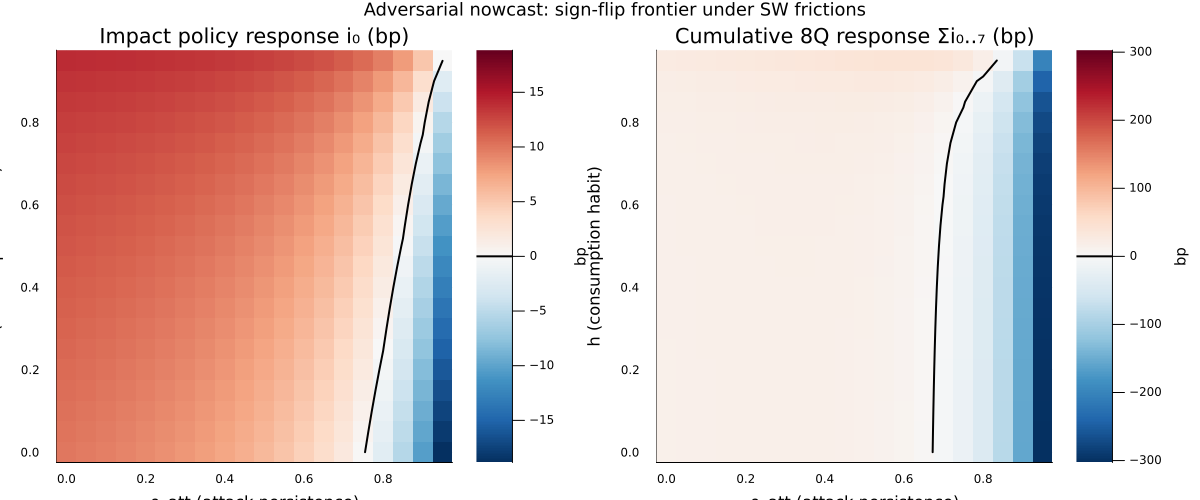
\includegraphics[width=0.9\textwidth]{../results/sweep_h_rho_att.png}
\caption{Two-dimensional parameter sweep over consumption habit \(h\) and attack persistence \(\rho_{\text{att}}\) under SW-posterior frictions. Left: impact response. Right: cumulative eight-quarter response. Black contour marks zero crossing.}
\label{fig:sweep}
\end{figure}

\subsection{Filtering reduces welfare loss with a tradeoff under normal conditions}\label{sec:welfare}

The single-gain perception filter introduces a robustness-vs-efficiency tradeoff familiar from \citet{svensson2003} and \citet{orphanides2007robust}. Under attack, filtering reduces welfare loss. Under normal conditions, it raises it, because the Fed becomes less responsive to legitimate gap movements. Table~\ref{tab:filter} reports three named regimes at empirical Phillips slope \(\kappa = 0.15\):

\begin{table}[h]
\centering
\small
\begin{tabular}{lccccc}
\toprule
Regime & \(K\) & \(L_{\text{no attack}}\) & \(L_{\text{attack}}\) & \(\Delta\) attack cost & Robustness gain \\
\midrule
Naive Fed & 1.00 & 2.95 & 9.59 & \(+6.64\) & baseline \\
Moderate filter & 0.50 & 3.06 & 7.43 & \(+4.37\) & \(+34\%\) \\
Policy-optimal filter & 0.025 & 4.62 & 4.86 & \(+0.23\) & \(+97\%\) \\
\bottomrule
\end{tabular}
\caption{Welfare loss by Fed filter regime at \(\kappa = 0.15\), SW-posterior frictions. Robustness gain is the percentage reduction in attack-induced welfare cost relative to naive Fed.}
\label{tab:filter}
\end{table}

Stochastic simulation (50 draws of 800-period paths) produces welfare estimates that are systematically 15--30\% higher than the analytical values (Table~\ref{tab:stoch}) but with the same ordering and comparable treatment effects. Standard errors are small relative to the welfare differences between regimes: the crossover between naive and policy-optimal filter is well-identified.

\begin{table}[h]
\centering
\small
\begin{tabular}{llrr}
\toprule
Regime & Attack & Mean \(L\) (analytical) & Mean \(L\) (stochastic, SE) \\
\midrule
Naive (\(K=1.00\)) & Off & \(2.95\) & \(3.83 \pm 0.07\) \\
Naive (\(K=1.00\)) & On & \(9.59\) & \(10.34 \pm 0.19\) \\
Policy-optimal (\(K=0.025\)) & Off & \(4.62\) & \(5.50 \pm 0.10\) \\
Policy-optimal (\(K=0.025\)) & On & \(4.86\) & \(5.76 \pm 0.10\) \\
\bottomrule
\end{tabular}
\caption{Analytical vs stochastic-simulation welfare estimates at \(\kappa = 0.15\). 50 draws, 800-period paths, 200-period burn-in. The simulations validate the ordering of the analytical estimates; the \(\sim 20\%\) gap reflects finite-sample variance not captured by the sum-of-squared-IRFs formula.}
\label{tab:stoch}
\end{table}

\subsection{The crossover threshold is robust at empirical Phillips slope}\label{sec:lambda}

The crossover probability \(p^*\) is the minimum perceived attack probability at which the policy-optimal filter dominates the naive Fed in expected welfare:
\[
p^* = \frac{L_{\text{no attack}}(K^*) - L_{\text{no attack}}(K = 1)}{\left[L_{\text{attack}}(K = 1) - L_{\text{attack}}(K^*)\right] + \left[L_{\text{no attack}}(K^*) - L_{\text{no attack}}(K = 1)\right]}.
\]

Table~\ref{tab:kappa_lambda} reports \(p^*\) across four welfare weights \(\lambda \in \{0.1, 0.25, 0.5, 1.0\}\) and three Phillips slopes.

\begin{table}[h]
\centering
\small
\begin{tabular}{lcccc}
\toprule
& \(\lambda = 0.10\) & \(\lambda = 0.25\) & \(\lambda = 0.50\) & \(\lambda = 1.00\) \\
\midrule
\(\kappa = 0.06\) (toy)         & \(44.3\%\) & \(45.0\%\) & \(39.2\%\) & \(41.4\%\) \\
\(\kappa = 0.15\) (empirical)   & \(25.7\%\) & \(25.8\%\) & \(26.1\%\) & \(26.6\%\) \\
\(\kappa = 0.20\) (empirical)   & \(21.7\%\) & \(21.8\%\) & \(21.9\%\) & \(22.2\%\) \\
\bottomrule
\end{tabular}
\caption{Crossover threshold \(p^*\) across Phillips slope and welfare weight. At empirical \(\kappa \in \{0.15, 0.20\}\), the crossover is largely independent of \(\lambda\). The toy calibration produces a wider range.}
\label{tab:kappa_lambda}
\end{table}

At the empirical Phillips slope, \(p^*\) varies by less than one percentage point across the \(\lambda\) range. The headline claim that filtering pays above a \(\sim 25\%\) attack probability is therefore robust to the choice of welfare weight within the conventional quadratic-loss form. We note that this sensitivity exercise varies the magnitude of \(\lambda\) but not the functional form of the welfare loss: asymmetric loss specifications, an explicit zero-lower-bound penalty, or interest-rate-smoothing preferences could shift the threshold further. The \(\kappa\) dependence is real, however: at the flat Phillips slope of the frictionless calibration (\(\kappa = 0.06\); Blakeslee 2025), the threshold is around \(40\%\); at \(\kappa = 0.20\) it drops to \(22\%\). We report the empirical-\(\kappa\) range \(22\)--\(26\%\) as the policy-relevant band.

\paragraph{Inflation-channel decomposition.}
Decomposing the welfare loss into variance-of-\(\pi\) and variance-of-gap contributions clarifies why steeper Phillips curves reduce the threshold. At \(\kappa = 0.15\), \(\mathrm{Var}(\pi)\) under naive Fed rises from \(2.86\) (no attack) to \(9.39\) (attack), while \(\mathrm{Var}(y^{\text{gap}})\) barely moves (\(0.19 \to 0.39\)). The attack's damage flows primarily through the inflation channel, which scales with \(\kappa\). Filtering reduces this pass-through. The cost of filtering under normal conditions (the Fed's loss of responsiveness to true gap movements) scales less aggressively with \(\kappa\). The benefit-cost ratio therefore rises with \(\kappa\), pushing the threshold down.

\section{The Strategic Attacker}\label{sec:attacker}

To make the attack endogenous, we equip the attacker with a utility function over the expected damage, a detection-probability cost, and a choice of magnitude and persistence. Let \(A = \sigma_{\text{att}}\) denote the attack magnitude and \(\rho = \rho_{\text{att}}\) the persistence. Detection probability is a stylized monotonic function
\begin{equation}\label{eq:det}
P_{\text{det}}(A, \rho) = 1 - \exp(-\gamma_d \, A^2 \, \rho),
\end{equation}
calibrated so that the baseline attack (\(A = 1, \rho = 0.8\)) has a 50\% detection probability. The attacker's expected utility is the undetected-adjusted damage, and we consider three alternative damage metrics:
\begin{itemize}
\item[(a)] cumulative negative policy-rate shift (attacker pushes rates down);
\item[(b)] inflation-variance damage (sum of squared IRFs of \(\pi\) attributable to the attack shock);
\item[(c)] output-gap-variance damage.
\end{itemize}

Table~\ref{tab:attacker} reports the attacker's optimum under naive and policy-optimal-filter Feds, across the three objectives.

\begin{table}[h]
\centering
\small
\begin{tabular}{llccc}
\toprule
Fed regime & Objective & \(A^*\) & \(\rho^*\) & E[damage] \\
\midrule
Naive (\(K = 1.00\)) & (a) cumulative \(|\Delta i|\) (bp) & 0.90 & 0.90 & 99.9 \\
Naive                & (b) \(\mathrm{Var}(\pi)\) damage    & 1.10 & 0.90 & 12.2 \\
Naive                & (c) \(\mathrm{Var}(y^{\text{gap}})\) damage & 1.10 & 0.90 & 0.17 \\
\midrule
Filter (\(K = 0.025\)) & (a) cumulative \(|\Delta i|\) (bp) & 0.90 & 0.90 & 19.2 \\
Filter                 & (b) \(\mathrm{Var}(\pi)\) damage    & 1.10 & 0.90 & 0.37 \\
Filter                 & (c) \(\mathrm{Var}(y^{\text{gap}})\) damage & 2.90 & 0.00 & 0.002 \\
\bottomrule
\end{tabular}
\caption{Attacker's optimal \((A^*, \rho^*)\) across three damage metrics and two Fed regimes. Objectives (a) and (b) give the same attack profile regardless of regime; the filter reduces expected damage without displacing the optimum. Objective (c) \emph{is} displaced by filtering, with the attacker switching to a high-magnitude, zero-persistence profile with near-zero realized damage.}
\label{tab:attacker}
\end{table}

Three findings. First, the attacker's optimum under objectives (a) and (b) is invariant to the Fed's filter regime: \((A^*, \rho^*) = (0.9, 0.9)\) under both naive and policy-optimal filter. The filter scales the damage surface without displacing the argmax. Second, the expected damage under filter is 80--97\% lower than under naive Fed across all three objectives. Third, for the output-gap-variance objective (c), filtering \emph{does} displace the attacker: the optimum shifts to a very high magnitude (\(A = 2.9\)), zero persistence, and a near-zero realized damage. Filtering here acts as both a damage reducer (for objectives a and b) and a partial deterrent (for objective c, where the attacker is pushed to a strategy that maximizes detection probability in exchange for minimal payoff).

Filtering operates as a damage reducer for the policy-rate-direction and inflation-variance objectives; the deterrence characterization applies only under the output-gap-variance objective. The broader lesson: whether filtering deters depends on what the attacker is trying to damage. If the attacker cares about the policy rate or inflation (the two metrics most visible to financial markets and the public), filtering reduces damage without shifting the attack; if the attacker cares specifically about output-gap volatility, filtering both reduces damage and shifts the attack profile. For a state adversary whose strategic objective is to distort US monetary policy or generate inflation volatility for geopolitical leverage, objectives (a) and (b) are the more plausible targets. Output-gap-variance damage (c) is a less visible and less directly leverageable outcome. The operative case for US defense design is therefore the damage-reducer case, and the defense ranking that follows treats it as canonical.

\section{Policy Implications}\label{sec:policy}

Earlier analysis (Blakeslee 2025) recommended three defense measures: cryptographic signatures on all third-party data feeds, uncertainty-adaptive Taylor coefficients, and a public provenance ledger. The strategic-attacker analysis developed here reorders these in terms of their leverage against the attacker's optimization problem:

\begin{enumerate}
\item \textbf{Provenance ledger} (first-order). Public logging of nowcast inputs enables crowd-sourced detection, as demonstrated by the American Sunlight Project's uncovering of the Pravda operation \citep{asp2025}. Detection latency feeds directly into \(\rho_{\text{att}}\), the attacker's most-leveraged variable. Operational caveats: upstream data providers' cooperation is required, and some inputs (card-swipe data, proprietary alt-data feeds) have contractual and privacy constraints that limit what can be logged publicly. Implementation timeline: 12--24 months for the Fed to negotiate provider agreements and build the audit infrastructure.

\item \textbf{Cryptographic signatures} (first-order). Signing at ingestion raises the cost of sustained attacks by making silent poisoning evident in the audit trail. This caps feasible \(\rho_{\text{att}}\) at a level set by the attacker's key-compromise budget. Operational caveat: the Fed's nowcast stack pulls from dozens of upstream providers of varying technical sophistication; smaller alt-data vendors would need support adopting hardware-security-module-based signing. Coordination with ECB and BoE would reduce per-provider adoption costs.

\item \textbf{Filter-based response} (second-order). Filtering is damage mitigation conditional on attack and (per Section~\ref{sec:attacker}) does not deter the attacker in the policy-rate-direction or inflation-variance cases. Its welfare benefit becomes positive when the Fed's perceived attack probability exceeds roughly \(22\)--\(26\%\) at empirical Phillips slope. This is within the range that security researchers treat as plausible for sustained adversarial activity against a high-value US target. Implementation timeline: immediate (it is an internal model parameter). Market-structure caveat: a visibly filtering Fed may face steeper market reactions when it eventually moves, because private agents' own nowcasts remain unfiltered. This is a classical credibility-vs-responsiveness tradeoff that any commitment to filtering would need to address.
\end{enumerate}

The first two measures attack the attacker's cost function and shift the feasible attack profile toward less damaging strategies. The third mitigates damage conditional on attack but does not change the attacker's incentives (except under objective c, noted above). The earlier equal treatment of these three measures is superseded by a clearer ordering: detection and signing are strategic-defense instruments; filtering is operational risk management.

\paragraph{On actionability of the \(25\%\) threshold.}
A Fed governor cannot credibly assert ``I believe \(P(\text{attack}) = 30\%\).'' The threshold is analytically useful but operationally abstract. A practical trigger framework would link it to observable indicators. Candidate red flags: divergence between the Fed's nowcast and comparable third-party nowcasts (Jefferies, Goldman, Evercore) that exceeds historical norms; detection by external audit (of the kind that uncovered the Pravda operation) of anomalous activity in upstream data providers; elevated geopolitical threat intelligence indicating active economic-statecraft operations against the US. Translating the \(25\%\) threshold into a staff-implementable rulebook is the natural next operational step.

\section{Limitations}\label{sec:limits}

\textbf{The perception filter is simplified.} A full Kalman filter would track multivariate uncertainty and use time-varying gains optimally under the full shock covariance matrix. The single-gain EWMA specification used here is a policy-tunable approximation; its advantage is interpretability and clean sweep. Section~\ref{sec:mmse} compares the policy-optimal \(K\) to the MMSE benchmark and documents the gap.

\textbf{Welfare is evaluated unconditionally.} The \(\lambda = 0.5\) baseline is consistent with the micro-founded derivation in \citet{woodford2003}, and Section~\ref{sec:lambda} confirms that the headline crossover threshold is robust to \(\lambda\) at empirical Phillips slopes.

\textbf{The attacker's information set is unspecified.} The strategic attacker here knows the Fed's filter parameters. A game-theoretic extension with incomplete information would be valuable. The framework of \citet{kamenica2011bayesian} Bayesian persuasion is the natural next step.

\textbf{Detection is purely probabilistic.} The cost function in equation~(\ref{eq:det}) is stylized. A richer specification would make detection depend on the Fed's filter output itself (anomalies flagged when raw and filtered signals diverge beyond a threshold), creating strategic complementarity between filtering and detection.

\textbf{The threat model omits multi-stakeholder dynamics.} Allied central banks (ECB, BoE, BoJ) run comparable nowcast operations; coordinated defense on provenance and signature standards would amplify protection but is outside the current model.

\textbf{The Fed's perception is bounded-rational.} Rational expectations hold for households and firms; the Fed alone is modeled as a bounded-rational filter. This asymmetry is tractable but shapes the results; a fully rational-expectations version with the Fed running a proper Kalman filter would shift the optimal \(K\) toward the MMSE value.

\section{Conclusion}

How much distortion can a persistent adversarial nowcast attack produce, and when should the Fed filter? Earlier analysis (Blakeslee 2025) demonstrated the attack mechanism with a frictionless three-equation DSGE and a knife-edge calibration. This brief rebuilds that analysis on a workhorse Smets--Wouters foundation and reaches two substantive revisions. The clean impact sign-flip of the earlier calibration does not survive consumption habit; under realistic frictions the attack's signature is a small initial hike followed by a drawn-out multi-quarter undershoot, harder to detect precisely because it is displaced in time. The cumulative footprint is nonetheless several times larger, and a cost-sensitive attacker pushes persistence rather than magnitude to its ceiling. At empirical Phillips-curve slopes, a Fed that perceives the probability of an active attack as exceeding roughly one in five should filter its nowcast signals heavily. Provenance ledgers and cryptographic signatures target the attacker's most-leveraged variable and are first-order defenses; filter-based responses are operational damage mitigation conditional on attack.

\paragraph{Code.} Reproduction code, interactive demo, and reference data are available in the companion repository.

\begin{thebibliography}{99}
\bibitem[Aoki(2003)]{aoki2003}
Aoki, K. (2003). On the optimal monetary policy response to noisy indicators. \emph{Journal of Monetary Economics}, 50(3), 501--523.

\bibitem[Aldasoro et al.(2024)]{aldasoro2024gen}
Aldasoro, I., Gambacorta, L., Korinek, A., Shreeti, V., \& Stein, M. (2024). Intelligent financial system: how AI is transforming finance. BIS Working Paper No.\ 1194.

\bibitem[American Sunlight Project(2025)]{asp2025}
American Sunlight Project. (2025). A pro-Russia content network foreshadows the automated future of info ops.

\bibitem[Bank for International Settlements(2024)]{bis2024}
Bank for International Settlements. (2024). Annual Economic Report 2024, Chapter III: AI and the economy.

\bibitem[Biggio and Roli(2018)]{biggio2018wild}
Biggio, B., \& Roli, F. (2018). Wild patterns: Ten years after the rise of adversarial machine learning. \emph{Pattern Recognition}, 84, 317--331.

\bibitem[Blanchard et al.(2013)]{blanchard2013news}
Blanchard, O.\ J., L'Huillier, J., \& Lorenzoni, G. (2013). News, noise, and fluctuations: An empirical exploration. \emph{American Economic Review}, 103(7), 3045--3070.

\bibitem[Boivin and Giannoni(2006)]{boivin2006}
Boivin, J., \& Giannoni, M.\ P. (2006). DSGE models in a data-rich environment. NBER Working Paper 12772.

\bibitem[Coibion and Gorodnichenko(2012)]{coibion2012}
Coibion, O., \& Gorodnichenko, Y. (2012). What can survey forecasts tell us about information rigidities? \emph{Journal of Political Economy}, 120(1), 116--159.

\bibitem[ECB(2024)]{ecb2024ai}
European Central Bank. (2024). The rise of artificial intelligence: benefits and risks for financial stability. Financial Stability Review, May 2024.

\bibitem[Galí(2008)]{gali2008}
Galí, J. (2008). \emph{Monetary Policy, Inflation, and the Business Cycle: An Introduction to the New Keynesian Framework}. Princeton University Press.

\bibitem[Galí and Gertler(1999)]{gali1999}
Galí, J., \& Gertler, M. (1999). Inflation dynamics: A structural econometric analysis. \emph{Journal of Monetary Economics}, 44(2), 195--222.

\bibitem[Kamenica and Gentzkow(2011)]{kamenica2011bayesian}
Kamenica, E., \& Gentzkow, M. (2011). Bayesian persuasion. \emph{American Economic Review}, 101(6), 2590--2615.

\bibitem[NewsGuard(2025)]{newsguard2025}
NewsGuard. (2025). A well-funded Moscow-based global ``news'' network has infected Western artificial intelligence tools worldwide with Russian propaganda.

\bibitem[Nimark(2008)]{nimark2008}
Nimark, K. (2008). Monetary policy with signal extraction from the bond market. \emph{Journal of Monetary Economics}, 55(8), 1389--1400.

\bibitem[Orphanides(2001)]{orphanides2001}
Orphanides, A. (2001). Monetary policy rules based on real-time data. \emph{American Economic Review}, 91(4), 964--985.

\bibitem[Orphanides(2003a)]{orphanides2003historical}
Orphanides, A. (2003a). Historical monetary policy analysis and the Taylor rule. \emph{Journal of Monetary Economics}, 50(5), 983--1022.

\bibitem[Orphanides(2003b)]{orphanides2003monetary}
Orphanides, A. (2003b). Monetary policy evaluation with noisy information. \emph{Journal of Monetary Economics}, 50(3), 605--631.

\bibitem[Orphanides and Williams(2007)]{orphanides2007robust}
Orphanides, A., \& Williams, J.\ C. (2007). Robust monetary policy with imperfect knowledge. \emph{Journal of Monetary Economics}, 54(5), 1406--1435.

\bibitem[Smets and Wouters(2007)]{smetswouters2007}
Smets, F., \& Wouters, R. (2007). Shocks and frictions in US business cycles: A Bayesian DSGE approach. \emph{American Economic Review}, 97(3), 586--606.

\bibitem[Steinhardt et al.(2017)]{steinhardt2017}
Steinhardt, J., Koh, P.\ W., \& Liang, P. (2017). Certified defenses for data poisoning attacks. \emph{Advances in Neural Information Processing Systems}, 30.

\bibitem[Svensson and Woodford(2003)]{svensson2003}
Svensson, L.\ E.\ O., \& Woodford, M. (2003). Indicator variables for optimal policy. \emph{Journal of Monetary Economics}, 50(3), 691--720.

\bibitem[Woodford(2003)]{woodford2003}
Woodford, M. (2003). \emph{Interest and Prices: Foundations of a Theory of Monetary Policy}. Princeton University Press.

\end{thebibliography}

\end{document}
